%\documentclass[aspectratio=43]{beamer}
\documentclass[aspectratio=169]{beamer}
\usepackage[english]{babel}
\usepackage[utf8]{luainputenc}
\usepackage[edges]{forest}
\usepackage{fontspec,array,listings,lstautogobble}

\usepackage{tikz}
\usetikzlibrary{chains,shapes.symbols,graphs,graphdrawing,automata,arrows.meta}
\usepackage{pgf-lookup-and-require-fix}
\usegdlibrary{trees,layered,force}

\forestset{
  directory tree/.style={folder,grow'=0,fit=band,edge={mLightBrown,densely dotted},font=\ttfamily\tiny,s sep=4pt,inner ysep=.1pt}
}
\tikzset{
  simple tag obj/.style={name=#1,fill=olive!50!black!50,regular polygon,regular polygon sides=5,label={north:#1}},
  simple commit obj/.style={circle,fill=mDarkTeal},
  simple tree obj/.style 2 args={name=#1,fill=mLightBrown,label={north:#1},
    append after command={
      \foreach \i/\j in {#2} {(#1) -- (\i) node[font=\tiny,sloped,inner ysep=.1pt,below,midway]{\j}}
    }
  },
  simple blob obj/.style={name=#1,draw,densely dashed,label={north:#1},font=\ttfamily\fontsize{4}{4}\selectfont,text width=44pt},
  every label/.style={font=\tiny,rotate=60,text width=4.7em,align=center},
  symref/.style={teal!66!black},
  TTfamily/.style={draw,text width=.85\textwidth,font=\ttfamily\tiny\bfseries},
  warning/.style={regular polygon,regular polygon sides=3,draw,
    red,node contents=!,inner sep=0pt,font=\scriptsize,
    append after command={node[right=1ex of \tikzlastnode,inner xsep=0pt,red] {#1}}
  },
  mLightBrown83/.style={mLightBrown!83!black},
  >=Latex,
  remote/.style={regular polygon,regular polygon sides=6,fill=teal},
  hint box/.style={fill=olive!20,draw=olive!50,rounded corners,text width=\textwidth,align=center},
}
\definecolor{cred}{HTML}{dc322f}
\definecolor{cgreen}{HTML}{859900}
\definecolor{cyellow}{HTML}{b58900}

\def\Q{\textbf{Q: }}
\def\A{\textbf{A: }}
\def\warning#1{\vrule height4ex width0ex \tikz\node[warning={#1}];}
\def\gitRebaseWarning{\warning{USE WITH CARE. Read git-rebase implications!}}
\def\LT{\textless}
\def\GT{\textgreater}
\def\hintBox#1{\tikz[remember picture,overlay]\node[hint box,anchor=south] at ([yshift=1in]current page.south) {#1};}

\lstset{autogobble}
\lstdefinestyle{bash}{
  language=bash,
  commentstyle=\color{cyellow},
  escapechar=`,
  basicstyle=\ttfamily\tiny\bfseries,
  breaklines=true,
  showspaces=false,
  framextopmargin=0pt,
  framexrightmargin=0pt,
  framexbottommargin=0pt,
  framexleftmargin=0pt,
}

\usetheme[usetotalslideindicator]{metropolis}
% ==== BEGIN THEME FIXES ====
\makeatletter
\let\@@TOC=\tableofcontents
\def\tableofcontents[#1]{\bgroup\parskip=0pt\@@TOC[#1]\egroup}
\makeatother
\AtBeginDocument{
  \setbeamertemplate{section in toc}[square]
  \setbeamertemplate{itemize items}{\raisebox{.5ex}{\rule{.5ex}{.5ex}}}
}
% ==== END THEME FIXES ====

\title{\uppercase{Git - There be dragons!}}
\subtitle{from \emph{(l)user} to \emph{r00t} in 60 minutes}
\author{Javier López-Gómez --- \protect{\tiny\url{https://jalopezg.dev/}}}
\institute{Senior Compiler Engineer ---Zimperium, Inc.}
\date{April 15th, 2024}
\titlegraphic{
\includegraphics[width=0.88in]{img/git-scm_logo_2x.png}}

\begin{document}

\maketitle
\begin{frame}{LICENSE}
  \centering This presentation can be redistributed and/or modified under the terms of CC-BY-NC 
\includegraphics[height=.5\baselineskip]{img/LICENSE.png} license.
\end{frame}
\begin{frame}{Agenda}
  \tableofcontents[hidesubsections]
\end{frame}

% ==== INTRODUCTION ====
\section{Introduction}

\begin{frame}{SCM/Revision control systems}
  ``Version control is a system that records changes to a file or set of files over time so that you can recall specific versions later (\ldots{}) if you screw things up or lose files, you can easily recover.'' [\texttt{https:///git-scm.org/}]\\[2em]
  
  What you get:
  \begin{itemize}
  \item Compare changes over time or revert files.
  \item See who introduced an issue.
  \item Make experimental changes (and merge them).
  \item \ldots{}
  \end{itemize}
\end{frame}

\begin{frame}{RCS models: centralized/distributed}
  \begin{columns}
    \column{.5\textwidth}
    \centering
    \tikz\graph[spring layout,nodes={remote,as=}] {
      a[fill=mDarkTeal] -- { b, c, d, e, f };
    };\par
    \textbf{Centralized:} Subversion (SVN), CVS\ldots{}

    \column{.5\textwidth}
    \centering
    \tikz\graph[spring layout,node distance=31pt,nodes={remote,as=}] {
      a -- { b, c -- { e -- h, g }, d -- { f, g } };
    };\par
    \textbf{Distributed:} git, Mercurial (hg)\ldots{}
  \end{columns}
\end{frame}

\begin{frame}{git - the stupid content tracker}
  \begin{center}
    \texttt{git != GitHub != GitLab}\ldots{}\\[4ex]
  \end{center}

  \only<1>{
  \begin{columns}
    \tikzset{forbidden/.style={forbidden sign,line width=.6ex,inner xsep=0pt,inner ysep=0pt,
        draw=red}}
    \column{.5\textwidth}
    \centering\tikz\node[forbidden]{
\includegraphics[width=.5in]{img/github-logo.png}};
    
    \column{.5\textwidth}
    \centering\tikz\node[forbidden]{
\includegraphics[width=.5in]{img/gitlab-logo.png}};
  \end{columns}
  }

  \only<2>{
  \begin{center}
    
\includegraphics[width=.5in]{img/git-scm_logo_2x.png}
  \end{center}
  Git: a distributed RCS.\par
  Started by Linus Torvalds; currently maintained by Junio C Hamano.
  }
\end{frame}

\begin{frame}{git - the stupid content tracker}
  \begin{itemize}
  \item \alert{150+} executable files; most symlinks to \texttt{/usr/bin/git} (à la \texttt{busybox}); some of them take lots of options! e.g. \texttt{git-log} parses 100+ options
  \item Divided into high level (porcelain) and low level (plumbing) commands
  \item Largely documented:\par
    {\ttfamily\small\$ basename --suffix=.1.gz /usr/share/man/man1/git* | xargs man | wc -l\\
      53260} (=870 pages PDF)
  \item Target of this talk: \emph{people using Git}
  \end{itemize}
\end{frame}

\begin{frame}{git 101}
  \centering
  \begin{tabular}{|l||>{\ttfamily\scriptsize}p{.5\textwidth}|}
    \hline
    Initialization & git clone\newline git init                   \\ \hline
    Interrogation  & git log\newline   git status\newline git diff\\ \hline
    Manipulation   & git add\newline   git commit                 \\ \hline
    Interaction    & git push\newline  git pull                   \\
    \hline
  \end{tabular}
\end{frame}

% ==== GIT ESSENTIALS ====
\section{Git essentials}

\begin{frame}{Working tree and .git/ directory (1/2)}
  \begin{columns}
    \column{.55\textwidth}
    \begin{description}[]
    \item[\texttt{.git/} directory:] contains Git administrative and control files.
    \item[Working tree:] the tree of checked out files.
    \end{description}

    \column{.45\textwidth}
    \centering
    \begin{forest} for tree={directory tree}
      [repository/
        [.git/
          [config] [HEAD] [\ldots]
        ]
        [Makefile] [main.cpp]
        [\ldots]
      ]
    \end{forest}
  \end{columns}
\end{frame}

\begin{frame}{Working tree and .git/ directory (2/2)}
  \begin{columns}
    \column{.55\textwidth}
    \begin{description}[]
    \item[Bare repository:] \alert{NO} working tree + \alert{NO} \texttt{.git/} directory sub-directory.\par
      Git files directly present in the directory.
    \end{description}

    \column{.45\textwidth}
    \centering
    \begin{forest} for tree={directory tree}
      [repository.git/
        [config] [HEAD] [\ldots]
      ]
    \end{forest}
  \end{columns}
\end{frame}

\begin{frame}{Objects, references and symrefs (1/3)}
  \begin{description}[]
  \item<1->[Object:] raw octets stored in Git; identified by its SHA-1.\par
    Types: \emph{commit}, \emph{tree}, \emph{blob}, \emph{tag}.
  \item<2->[Ref(erence):] a name that points to an object. Hierarchical namespace rooted at \texttt{refs/}
  \item<3->[Symref:] a ref that points to another ref, e.g. HEAD.
  \end{description}

  \begin{center}
    \only<3->{\tikz[every node/.style={font=\tiny,on chain,join},
      every join/.style={->},start chain=going below,node distance=20pt] \path
        node [symref] {HEAD}
        node        {refs/heads/master}
        node [draw] {770fcfa540f5f5d1f49570b9d09320c7a7b7e879 (commit)};}
  \end{center}
\end{frame}

\begin{frame}{Objects, references and symrefs (2/3)}
  \begin{columns}
    \column{.5\textwidth}
    The contents of an object depend on its type:
    \begin{description}[]
    \item<1->[Blob:] raw data; stores file contents.
    \item<2->[Tree:] directory contents.
    \item<3->[Commit:] information about a revision.
    \item<4->[Tag:] ref pointing to a commit + message + PGP signature (optional).
    \end{description}

    \column{.5\textwidth}
    \centering
    \tikz[every label/.style={font=\tiny,rotate=0}]{
      % blob objects
      \node[simple blob obj={9355a87}] {\#\\ \# /etc/hosts: \ldots{}};
      \node[simple blob obj={0632e41},below=24pt of 9355a87] {\# Generated by NetworkManager\\ search arcos.\ldots{}};
      % tree
      \draw<2->[->] node[simple tree obj={3814f01}{9355a87/hosts,
                                        0632e41/resolv.conf},
        below=12pt of 9355a87,xshift=-70pt]{};
      % commit chain
      \draw<3->[->] graph[tree layout,grow'=up,nodes={simple commit obj,as=}] {
        a <- aa <- aaa[label={left:efa21b0},desired at={(-90pt,-23pt)}] <- aaaa;
      }
      (aaaa) |- (3814f01);
      % tag
      \draw<4->[<-] (aa) -- ++(-30pt,0pt) node[simple tag obj={a27c52b}]{};
    }
  \end{columns}
\end{frame}

\begin{frame}{Objects, references and symrefs (3/3)}
  Typically, objects can be reached given a ref (but not always).
  \begin{columns}
    \column{.5\textwidth}
    \begin{center}
      \tikz\graph[tree layout,grow'=up,nodes={simple commit obj,as=}]{
        a -- { b -- c[red],
          d -- e -- f[label={north:refs/heads/master}] };
        };
    \end{center}\par
    \textbf{Unreachable object:} an object which is not reachable from any reference.

    \column{.5\textwidth}
    \vrule height .117\textheight width0pt
    \begin{center}
      \tikz\graph[tree layout,grow'=up,nodes={simple commit obj,as=}]{
        a -- b -- c[label={north:refs/heads/master}];
        d[red];
        };
    \end{center}\par
    \textbf{Dangling object:} not reachable even from other unrechable objects.
  \end{columns}
  
  \hfill {\tiny More at \texttt{gitglossary(7)}}
\end{frame}

\begin{frame}{Project history, branches and tags}
  \begin{columns}
    \column{.67\textwidth}
    \only<1->{Commit objects form a DAG (they point to their parents). This DAG is known as the history of a project.\\[-.6em] \rule{1in}{.1pt}\\[.3em]}
    \only<2-4>{\textbf{Branch:} an active line of development; \emph{tip:} the most recent commit.\\[.5em]}
    \only<3-4>{\textbf{(Branch) head:} a reference to the tip of a branch.\par Local heads at: \texttt{refs/heads/}.\\[.5em]}
    \only<4>{\textbf{Remote-tracking branch:} a ref to a remote head; follow changes from another repository.\par At \texttt{refs/remotes/*/}.}

    \only<5>{\textbf{Merge commit:} a commit object that has $\geq 2$ parents.\\[.5em]}
    \only<5>{\textbf{Octopus:} a merge that has $> 2$ parents.}

    \column{.33\textwidth}
    \tikz\graph[layered layout,grow'=down,level distance=2em,
              nodes={simple commit obj,as=}]{
      a <- aa[mLightBrown] <- { b <- bb <- bbb[label={70:refs/heads/foo}],
                                c <- cc[label={135:refs/remotes/origin/master}] }
        <- aaa[red] <- aaaa[label={north:refs/heads/master}];
    };
  \end{columns}
\end{frame}

\begin{frame}{The ``index'' (cache) file}
  \textbf{Short story:} basically, it is the staging area for the next commit.\\[1em]

  \begin{itemize}[<+->]
  \item ``A collection of files with stat information, whose contents are stored as objects.'' [\texttt{gitglossary(7)}]
  \item For each file, it stores \LT object SHA-1\GT\ \LT attributes\footnote{Last modified time, size, etc.}\GT\\
    \tikz\node[TTfamily]
              {100644 01cb7066623241a0e5714a6630f0355eb0c80de4 0\ \ \ \ .gitignore\\
                \ldots{}\\
                100644 94fbec4cf383e9122c22d60cfad91b3c897e2c63 0\ \ \ \ slides.tex};
  \item Changes to the working tree found by comparing these attributes.
  \item Entries may be updated (\texttt{git add}) and new commits may be created from the index.
  \end{itemize}
\end{frame}

\begin{frame}{Other definitions (1/3)}
  \textbf{Fast-forward:} a special type of merge; given two heads $A$ and $B$, merging $B$ into $A$ is considered fast-forward if $merge\_base(A, B) == A$, i.e. $A$ is ancestor of $B$.\\[1em]
  \begin{columns}
    \tikzset{every label/.append style={text width=}}
    \column{.5\textwidth}
    \begin{center}
      \tikz\graph[tree layout,grow'=up,level distance=7pt,
        nodes={simple commit obj,as=}] {
      a <- aa[red,label={north:A}] <-
      {[nudge right=3ex]
        c <- cc <- ccc[label={north:B}] };
      };
    \end{center}\par
    Fast-forward (update ref only!)

    \column{.5\textwidth}
    \vrule height .067\textheight width0pt
    \begin{center}
      \tikz\graph[tree layout,grow'=up,level distance=7pt,
        nodes={simple commit obj,as=}] {
      a <- aa[red] <-
      { b[label={north:A}],
        c <- cc <- ccc[label={north:B}] }; 
      };
    \end{center}\par
    Non fast-forward (requires a merge)
  \end{columns}
\end{frame}

\begin{frame}{Other definitions (2/3)}
  \begin{columns}
    \tikzset{every label/.append style={text width=}}
    \column{.5\textwidth}
    \begin{description}[]
    \item<1-5>[HEAD:] symref that dereferences to the current checked-out head.
    \item<2-5>[Detached HEAD:] HEAD may also point at an arbitrary commit, i.e. ``detached'' from any branch. You may make commits in this state, but\ldots{}
    \end{description}
    \only<6>{if HEAD is made to point somewhere else, they will become unreachable (and eventually deleted by the GC). \alert{Create a ref to avoid this!} }
    
    \column{.5\textwidth}
    \centering
    \tikz{
      \graph[tree layout,grow'=up,nodes={simple commit obj,as=}] {
      a <- aa[label={135:c864ac8}] <- aaa <- aaaa[label={north:refs/heads/master}];
      };
      % commit chain; head detached at c864ac8
      {[simple commit obj/.append style={at end}]
        \draw<3->[<-] (aa) -- ++(-3em,2em) node (b)[simple commit obj]  {};
        \draw<4->[<-] (b)  -- ++(0ex,2em)  node (bb)[simple commit obj] {};
        \draw<5->[<-] (bb) -- ++(0ex,2em)  node (bbb)[simple commit obj]{};
      }
      
      \foreach \i [count=\c] in {aaaa,aa,b,bb,bbb,aaaa}
        \draw<\c>[<-] ([xshift=-14pt,yshift=1pt]\i.north) to [bend left] node[symref,at end,above] {HEAD} ++(-10pt,15pt);
    }
  \end{columns}
\end{frame}

\begin{frame}{Other definitions (3/3)}
  \textbf{Reflog:} stores the local history of a ref - more on this later!\\[1em]

  \begin{itemize}
  \item What was \texttt{HEAD} pointing at before the last change?
  \item What did \texttt{refs/heads/foo} pointed at two weeks ago?
  \end{itemize}
\end{frame}

% ==== [(l)user] PORCELAIN ====
\section{\emph{[(l)user]} Porcelain}

\begin{frame}{Simple (and incomplete) FSM}
  \centering
  \tikz[shorten >=1pt,node distance=74pt,every node/.style={font=\tiny},
    every state/.style={white,draw=mDarkTeal!74!black!77,top color=mDarkTeal!74!black!34,bottom color=mDarkTeal!74!black!73},
    initial text={git init/git clone},
    fwd/.style={->,sloped,bend left=10,above},
    bwd/.style={<-,sloped,bend right=10,below}]
       {
         \node[state,initial] (clean)                         {Clean WD};
         \node[state]         (dirty)  [above right=of clean] {Dirty WD};
         \node[state]         (staged) [right=of dirty]       {Staged};
         \node[state]         (merge) [below right=of clean]  {Merging};
         
         \path (clean) [fwd] edge node {[make changes]} (dirty)
                       [bwd] edge node {git checkout}   (dirty)
                       [fwd] edge node {git pull/git merge}   (merge)
                       [bwd] edge node {git merge --continue} (merge)
               (dirty) [fwd] edge node {git add}        (staged)
                       [bwd] edge node[text width=5em] {git rm --cached\\ git reset}      (staged)
              (staged) [fwd,bend left=20] edge node[text width=5em] {git commit\\ git reset --hard}       (clean)
                       [bwd,bend left=37] edge node {git rm/git mv} (clean);
         \path[->] (clean)   edge [loop above] node[text width=3em] {git push\\ git fetch}      ()
                             edge [loop below] node {git clean}     ();
         \path[->] (dirty)   edge [loop above] node {git diff}          ()
                   (staged)  edge [loop above] node {git diff --cached} ();
       }
\end{frame}

\begin{frame}{Init/Clone a repository}
  To get started, you can either
  \begin{itemize}
  \item Create an empty repository, e.g.\\
    \tikz\node[TTfamily]
              {\$ git init [--bare] \~{}/foo/};

  \item Obtain a copy of a remote repository\footnote{The \texttt{--depth} option creates a shallow clone (history pruned). To unshallow run \texttt{git pull --unshallow}.}, e.g.\\
    \tikz\node[TTfamily]
              {\$ git clone [--depth=1] https://earth/public/repo.git/};
  \end{itemize}
\end{frame}

\begin{frame}[fragile]{Overview of branches}
  \begin{lstlisting}[style=bash]
    # Create a branch started off from 'HEAD'
    $ git branch foo HEAD
    $ git checkout foo
    Switched to branch 'foo'

    $ git checkout -b foo HEAD # Shorthand for the above commands`\pause`

    # Create an orphan branch (new totally disconnected history)
    $ git checkout --orphan foo HEAD`\pause`

    $ git branch -d foo      # Delete a branch
    $ git branch -m foo bar  # Move/rename a branch

    # List branches
    $ git branch --verbose
    * `{\color{cgreen}foo}`    d7832a7f Closes issue #17
      master 99446829 Closes issue #16`\pause`

    # Merge a branch
    $ git merge foo
    # Resolve conflicts + 'git add <pathspec> ' + 'git merge --continue'
    # or 'git merge --abort'
  \end{lstlisting}
\end{frame}

\begin{frame}{Working with remotes (1/4)}
  Git can manage remote sites (remotes\footnote{See \texttt{git-remote(1)} for more information.}) whose branches you track.
  \begin{columns}
    \column{.55\textwidth}
    \begin{itemize}
    \item Supports http[s]://, ssh://, git:// and file://.
    \item \texttt{git-clone} automatically adds the remote \emph{origin} (the URL you cloned)
    \item May have different push/fetch URLs
    \item<2> \alert{REMEMBER:} Git is distributed
    \end{itemize}

    \column{.45\textwidth}
    \centering
    \tikz[every label/.style={font=\tiny}]
         {
           \graph[layered layout,grow=up,node distance=31pt,nodes={remote,as=}]
                 { a[fill=mDarkTeal,label=below:local copy] -- { b, c, d, e, f } };
           \draw<2> (c) -- ++(0pt,3em) node(g)[remote,anchor=south]{}
                 (e) to [bend left] (g)
                 (f) to [bend left] (g);
         }
  \end{columns}
\end{frame}

\begin{frame}{Working with remotes (2/4)}
  \begin{itemize}[<+->]
  \item Remotes may be added with \texttt{git-remote}, e.g.\\[1ex]
    \tikz\node[TTfamily]
              {\$ git remote add earth https://earth/public/repo.git/};\par
    Default is to track all branches\footnote{Otherwise, see \texttt{-t \LT branch\GT}}.
  \item \texttt{git-push} pushes refs (+ objects) to a remote, e.g.\\[1ex]
    \tikz\node[TTfamily]
              {\$ git push earth master};
  \item \texttt{git-fetch} fetches refs (+ objects) from a remote, e.g.\\[1ex]
    \tikz\node[TTfamily]
              {\$ git fetch earth master};\par
    Fetched refs will be in \texttt{refs/remotes/earth/*}.
  \item \texttt{git-pull} is equivalent to \texttt{git fetch} + \texttt{git merge FETCH\_HEAD}
  \end{itemize}
\end{frame}

\begin{frame}{Working with remotes (3/4)}
  Trying a {\ttfamily\scriptsize\$ git push earth master}
  \begin{itemize}[<+->]
  \item On the remote end: receive object pack + update refs
  \item Synching only requires commit 63feb3c
  \item \alert{Non-FF}. If earth updates refs/heads/master, commit 9f7f586 is lost!\par
    Typically, remotes will deny non-fast-forward pushes\footnote{See the \texttt{-f} git-push(1) option and \texttt{receive.denyNonFastForwards}.}
  \end{itemize}\vfill

  \only<1-3>{\begin{columns}
    \tikzset{every label/.style={font=\tiny}}
    \column{.5\textwidth}
    \centering
    \tikz\graph[tree layout,grow'=up,nodes={simple commit obj,as=}]
               { a[label=left:7d050cf] <- aa[opacity=.5,label=left:63feb3c,
                   label=above:refs/heads/master]};\par
    Local
    \column{.5\textwidth}
    \centering
    \tikz{
      \graph[tree layout,grow'=up,nodes={simple commit obj,as=}]
            { a[label=left:7d050cf] <- b[mLightBrown,label=left:9f7f586,
                label=above:refs/heads/master]};
      \draw<2->[<-,densely dashed] (a) -- ++(4ex,4ex)
            node[simple commit obj,anchor=south west,opacity=.5,label=right:63feb3c]{};
    }\par
    Remote \texttt{earth}
  \end{columns}}

  \only<4>{\tikz\node[TTfamily]{
    {\color{cred}! [rejected]}\ \ \ \ \ \ \ \ master -\GT master (non-fast-forward)\\
    \color{cred}error: failed to push some refs to '\ldots'};
  }
\end{frame}

\begin{frame}{Working with remotes (4/4)}
  Trying a {\ttfamily\scriptsize\$ git pull earth master}\footnote{The merge might be avoided; see the \texttt{--rebase} option.}\vfill

  \begin{columns}
    \tikzset{every node/.style={font=\tiny},
      every label/.style=}
    \column{.5\textwidth}
    \centering
    \tikz{
      \graph[tree layout,grow'=up,nodes={simple commit obj,as=}]
            { a[label=left:7d050cf] <- aa[opacity=.5,label=left:63feb3c] };
      \draw<2->[<-] (a) -- ++(4ex,4ex)
            node (9f7f586) [simple commit obj,mLightBrown,anchor=south west,label=right:9f7f586]{};
      \draw<3>[<-] (aa) -- ++(0ex,4ex)
           node (618c1ca) [simple commit obj,anchor=south,label=right:618c1ca]{}
                (9f7f586) -- (618c1ca);
      \path<1-2> node[above=0pt of aa]                  {master};
      \path<2->  node[above=0pt of 9f7f586,anchor=west] {FETCH\_HEAD -\GT{} earth/master};
      \path<3>   node[above=0pt of 618c1ca]             {master};
    }\par
    Local
    \column{.5\textwidth}
    \centering
    \tikz{
      \graph[tree layout,grow'=up,nodes={simple commit obj,as=}]
            { a[label=left:7d050cf] <- b[mLightBrown,label=left:9f7f586,
            label=above:refs/heads/master] };
    }\par
    Remote \texttt{earth}
  \end{columns}
\end{frame}

\begin{frame}{Bug hunting}
  Git helps you to find bugs (and their authors)\ldots\\[1em]
  \begin{description}[]\itemsep=2em
  \item[git-bisect(1)] uses binary search to find a ``bad'' commit\\[1ex]
    \tikz\node[TTfamily]
              {\$ git bisect start HEAD v1.2 {\color{cyellow}\# HEAD is bad, v1.2 is good}\\[1ex]
              \$ git bisect [good|bad] {\color{cyellow}\# Manually mark it as working/broken}\\
              \ldots\\
              \$ git bisect run my\_script arguments {\color{cyellow}\# Or automatically (good if \$? = 0)}\\[1ex]
              \$ git bisect reset};

  \item[git-blame(1)] annotates each line of a file with revision information\\[1ex]
    \tikz\node[TTfamily]
              {\$ git blame README.md\\
                63feb3c8 (jalopezg 2019-01-18 19:36:40 +0100 1) \GT This file was created by \ldots\\
              ded8aa43 (jalopezg 2019-01-22 20:18:04 +0100 2) foo};
  \end{description}
\end{frame}

\begin{frame}{Specifying revisions (1/2)}
  Some Git commands take symbolic revision parameters (names specific commit or all commits reachable from that commit)\footnote{This is an overview; see gitrevisions(7) for the complete list.}.

  \begin{description}[]
  \item[\LT sha1\GT] SHA-1 object name, or a non-ambiguous leading substring.
  \item[\LT refname\GT] A ref name, e.g. refs/heads/master. Search order: {\ttfamily\scriptsize \$GIT\_DIR/\LT refname\GT, refs/, refs/tags/, refs/heads/, refs/remotes/, refs/remotes/\LT refname\GT/HEAD}.
  \item[\LT refname\GT@\{\LT n\GT\}] The n-th prior value of that ref.
  \item[\LT rev\GT\^{}] The first parent.
  \item[\LT rev\GT\~{}\LT n\GT] The n-th generation ancestor.
  \item[\LT rev\GT:\LT path\GT] Names the blob or tree of \LT rev\GT.
  \end{description}
\end{frame}

\begin{frame}{Specifying revisions (2/2)}
  Specifying ranges:

  \begin{description}[]
  \item[\^{}\LT rev\GT] Exclude commits reachable from \LT rev\GT.
  \item[\LT rev1\GT..\LT rev2\GT] A shorthand for \^{}rev1 rev2, i.e. commits reachable from rev2, but not from rev1, or $\big(rev1,\ rev2\big]$
  \item[\LT rev1\GT...\LT rev2\GT] Commits reachable either from rev1 or rev2, but not from both.
  \end{description}
\end{frame}

% ==== [sudoer] MORE PORCELAIN ====
\section{\emph{[sudoer]} More porcelain}

\begin{frame}[fragile]{Save/Restore a dirty working directory}
  \texttt{git-stash(1)} saves the current state of the working directory + the index, and goes back to a clean WD.

  Saved changes can be restored with {\ttfamily\scriptsize\$ git stash pop}. Git-stash stack can be dumped by {\ttfamily\scriptsize\$ git stash list}.
  \pause

  \begin{lstlisting}[style=bash]
    $ echo foo > README.md
    $ git status
    On branch foo
    Changes not staged for commit:
    ``        `{\color{cred}modified:   README.md}\pause`

    $ git stash
    Saved working directory and index state WIP on foo: 9f7f586 README.md has been added
    $ git status
    On branch foo
    nothing to commit, working tree clean`\pause`

    $ git stash pop
    On branch foo
    Changes not staged for commit:
    ``        `{\color{cred}modified:   README.md}`
    Dropped refs/stash@{0} (35365e0c188e877ded1ecdd8190ec5bb1b6c2c1b)
  \end{lstlisting}
\end{frame}

\begin{frame}{Applying changes from other branches}
  \begin{columns}
    \column{.55\textwidth}
    \texttt{git-cherry-pick(1)} apply the changes introduced by the given commits, e.g.\par
    {\ttfamily\scriptsize\$ git cherry-pick 9f7f586}.\\[1em]
    The patch may not apply cleanly; if that is the case, you are required to resolve conflicts

    \column{.45\textwidth}
    \centering
    \tikz[every label/.style={font=\tiny}]{
      \graph[tree layout,grow'=up,nodes={simple commit obj,as=}]
            { a <- aa <- { b <- bb <- bbb[mLightBrown,label=left:9f7f586] <- bbbb[label=90:master],
                          c <- cc }
            };
      \draw<2>[<-] (cc) -- ++(0em,2.6em)
                   node(ccc)[simple commit obj,mLightBrown83,label=right:0c151e4]{};
      \foreach \i [count=\c] in {cc,ccc} \path<\c> node[above=0pt of \i,font=\tiny]{foo};
    }
  \end{columns}
\end{frame}

{
\tikzset{every label/.style={font=\tiny},
        commit 1/.style={simple commit obj,fill=teal},
        commit 2/.style={simple commit obj,fill=teal!74},
        commit 3/.style={simple commit obj,fill=teal!56}}
\begin{frame}{Rebase (+ interactive rebase!) (1/4)}
  Sometimes you fork a branch and it becomes outdated w.r.t. its parent. Quite probably, you would merge the parent branch.\par
  \begin{center}
    \tikz[hole/.style={densely dotted},
          merge/.style={simple commit obj,mLightBrown}]{
      \graph[tree layout,grow'=right,nodes={simple commit obj,as=}] {
        a <- aa[red] <- { [nudge down=3ex] b[label=above:A] <- bb[label=above:B] <- bbb[label=above:C] }
      };
      \draw<2->[<-] (aa) -- ++(3ex,3ex) node(c)[commit 1]{} -- ++(3ex,0ex) node(cc)[commit 2]{};
      \draw<2->[hole] (cc) -- ++(5ex,0ex) node(ccc)[commit 3]{};
      \draw<3->[<-] (bbb) -- ++(5ex,0ex) node(bbbb)[merge]{}
                    (ccc) -- (bbbb);
      \draw<4->[hole] (ccc) -- ++(10ex,0ex) node(cccc)[simple commit obj]{}
                    (bbbb) -- ++(10ex,0ex) node(bbbbb)[merge]{};
      \draw<4->[<-] (cccc) -- (bbbbb);
      % branch heads
      \foreach \i/\j/\k in {1/aa/master,1-2/bbb/topic,
                          2-3/ccc/master, 3/bbbb/topic,
                          4/cccc/master,4/bbbbb/topic}
        \path<\i> node[right=0pt of \j,font=\tiny]{\k};
    }
  \end{center}
  
  \onslide<5>{
    This clutters project history. Reapplying \texttt{topic} commits on top of \texttt{master} is better!\par
    \begin{center}
    \tikz\graph[tree layout,grow'=right,nodes={simple commit obj,as=}] {
        a <- aa[red] <- c[commit 1] <- cc[commit 2] <- ccc[commit 3,label=right:master]
            <- { [nudge down=3ex] b[label=above:A'] <- bb[label=above:B'] <- bbb[label=above:C',label=right:topic] }
      };
    \end{center}

    \tikz\node[TTfamily]
              {{\color{cyellow}\# Assuming that 'topic' is the current branch, this gives the result above}\\
              \$ git rebase master};
  }
\end{frame}

\begin{frame}{Rebase (+ interactive rebase!) (2/4)}
  It is one of the most powerful Git commands. In fact, it can be used to rewrite project history (next slide).\par\pause
  If there are conflicts, you will have to resolve them (as in merge).\pause

  \warning{\texttt{GIT-REBASE(1)} IMPLICATIONS:}
  \begin{itemize}
  \item Requires rewriting commits and is \alert{PROBLEMATIC} if you already pushed those objects
  \item You can break things: \alert{YOU HAVE BEEN WARNED!}
  \item If you ever force-push a rebased branch, others will have to fix their history. See git-rebase(1), section ``RECOVERING FROM UPSTREAM REBASE''.
  \end{itemize}
\end{frame}

\begin{frame}[fragile]{Rebase (+ interactive rebase!) (3/4)}
  \texttt{git-rebase(1)} has an interactive mode in which you can edit/reorder/remove the commits which are rebased.\\ It is very common to rewrite part of a branch to have a more meaningful history, e.g.

  \begin{center}
    \tikz\graph[tree layout,grow'=right,nodes={simple commit obj,as=}] {
        a <- aa[red] <- { c <- cc[label=right:master],
            b <- bb[label=below:\LT after-this-commit\GT]
              <- bbb[commit 1,label=above:A] <- bbbb[commit 2,label=above:B] <- bbbbb[commit 3,label=above:C,label=right:topic] }
      };
  \end{center}

  \begin{lstlisting}[style=bash]
    # This fires up an editor and gives you the chance to edit the commit list before they are applied (commits A, B and C)
    $ git rebase -i <after-this-commit>
  \end{lstlisting}

  \gitRebaseWarning
\end{frame}
}

\begin{frame}{Rebase (+ interactive rebase!) (4/4)}
  \centering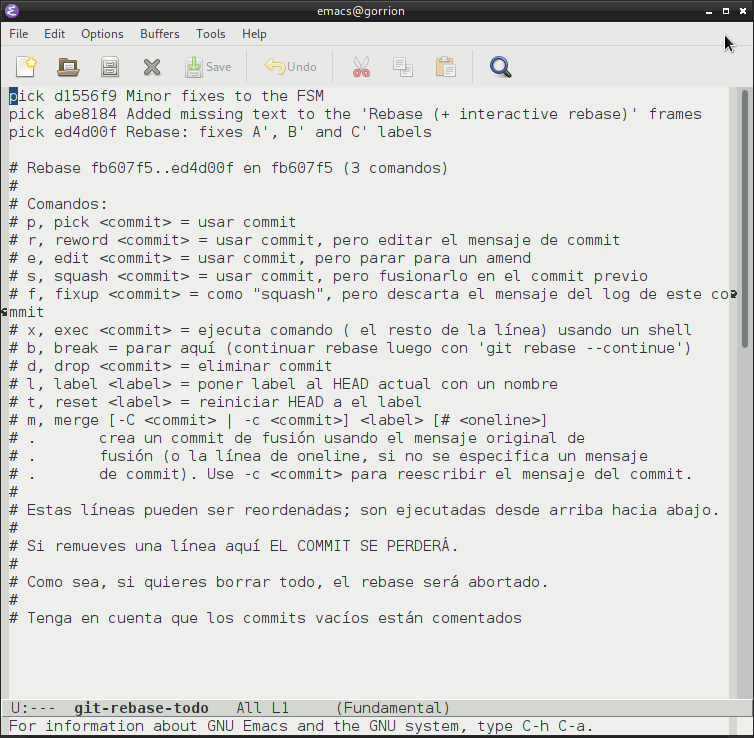
\includegraphics[height=.78\textheight]{img/git-rebase_-i.png}
\end{frame}

\begin{frame}[fragile]{More about fixing history (1/2)}
  So common that \texttt{git-commit(1)} has the \texttt{--squash} and \texttt{--fixup} options. They mark commits to be automatically squashed. Rewriting occurs after a {\ttfamily\scriptsize\$ git rebase --autosquash}.
  \pause
  \begin{lstlisting}[style=bash]
    $ git log --oneline
    e7a2019 (HEAD -> master) Any other changes
    9f7f586 Added README.md
    02a7fb9 Added bar.txt`\pause`

    $ echo foo >> README.md && git commit -a --fixup 9f7f586
    $ git log --oneline
    24a54df (HEAD -> master) fixup! Added README.md
    e7a2019 Any other changes
    9f7f586 Added README.md
    02a7fb9 Added bar.txt`\pause`

    $ git rebase -i --autosquash 02a7fb9
    Successfully rebased and updated refs/heads/master.
    $ git log --oneline
    528efb7 (HEAD -> master) Any other changes
    a59735c Added README.md
    02a7fb9 Added bar.txt
  \end{lstlisting}

  \gitRebaseWarning
\end{frame}

\begin{frame}{More about fixing history (2/2)}
  If you only need to rewrite the last commit use\\ {\ttfamily\scriptsize\$ git commit --amend}

  \gitRebaseWarning
\end{frame}

\begin{frame}{git filter-branch}
  \Q I know how to rewrite commits. Can I automate the process?\\
  \pause
  \A \texttt{git-filter-branch(1)} lets you rewrite branches, applying filters to modify each tree/information about each commit, e.g. \\[1em]

  \tikz\node[TTfamily]
            {\$ git log --oneline\\
            {\color{cyellow}92cb761} (HEAD -\GT{} foo) Added nsswitch.conf\\
            {\color{cyellow}9f7f586} Added README.md\\
            {\color{cyellow}02a7fb9} (bar) Added bar.txt\\[1ex]
            \$ git filter-branch --msg-filter 'sed -e "s/Added \textbackslash([[:graph:]]*\textbackslash)\$/\textbackslash{}1 has been added/"' foo\\[1ex]
            \$ git log --oneline\\
            {\color{cyellow}6e9fbd6} (HEAD -\GT{} foo) nsswitch.conf has been added\\
            {\color{cyellow}63feb3c} README.md has been added\\
            {\color{cyellow}2fe54f3} bar.txt has been addded};

  \gitRebaseWarning
\end{frame}

\begin{frame}{Comparing branches}
  \Q Can I see where each of the given branches is w.r.t. others?\\
  \pause
  \A \texttt{git-show-branch} is your friend. Also, \texttt{git log --graph --oneline \ldots}\\[1em]

  \tikz\node[TTfamily]
            {\$ git show-branch master foo\\
            {\color{cred}!} [master] Added README.md\newline
            \phantom{!}{\color{cgreen}*} [foo] Added nsswitch.conf\newline
            \phantom{!*}{\color{cyellow}!} [bar] Added bar.txt\\
            ---\newline
            \phantom{+}{\color{cgreen}*}\phantom{+} [foo] Added nsswitch.conf\\
            {\color{cred}+}{\color{cgreen}*}\phantom{+} [master] Added README.md\\
            {\color{cred}+}{\color{cgreen}*}{\color{cyellow}+} [bar] Added bar.txt\\[1ex]
            \# To include all remote-tracking and local branches:\\
            \$ git show-branch --all};
\end{frame}

\begin{frame}{Share by other means}
  TAR or ZIP archives of a particular tree can be created by \texttt{git-archive(1)}, e.g.\\[1ex]
    \tikz\node[TTfamily]
            {\$ git archive --format=tar --prefix=foo/ -o foo.tar.gz master};\\[2em]
            
  Git also can generate an archive of packed objects and references to be imported into a repository (useful if machines are not directly connected), e.g.\\[1ex]
    \tikz\node[TTfamily]
            {[alice@earth \~{}]\$ git bundle create /tmp/foo-master.git master\\
            \# /tmp/foo-master.git is copied to moon by some means.\\[1ex]
            [bob@moon \~{}]\$ git clone -b master \~{}/foo-master.git\\[1ex]
            \# Or if the repository already exists\ldots{}\newline
            [bob@moon \~{}]\$ git remote add foo-bundle \~{}/foo-master.git\newline
            [bob@moon \~{}]\$ git pull foo-bundle master};
\end{frame}

\begin{frame}{ReReRe}
  ``git-rerere - Reuse recorded resolution of conflicted merges''
  \\[1em]
  \alert{FYI, see the \texttt{git-rerere(1)} manual page.}
\end{frame}

% ==== [r00t] PLUMBING ====
\section{\emph{[r00t]} Plumbing}

\begin{frame}{Repository layout}
  \begin{columns}
    \column{.5\textwidth}
    \only<1>{\begin{description}[]
      \item[objects/:] the object store.
      \item[objects/{[0-9a-f][0-9a-f]}/:] loose objects.
      \item[objects/pack/:] object packs (store many objects in compressed form).
      \item[refs/:] references are stored in subdirectories of this directory.
      \item[packed-refs:] the same as refs/ but in a more efficient way.
      \item[HEAD:] the HEAD symref.
    \end{description}}
    \only<2>{\begin{description}[]
      \item[config:] repository specific configuration file.
      \item[hooks/:] (described later).
      \item[index:] the ``index'' file.
      \item[info/:] additional information, e.g. \texttt{info/grafts}.
      \item[logs/:] reflogs are stored here.
      \item[shallow:] similar to \texttt{info/grafts} but internally used for shallow clones.
    \end{description}}
    
    \column{.5\textwidth}
    \centering
    \begin{forest} for tree={directory tree}
      [repository/
        [.git/
          [objects/
            [pack/] [{[0-9a-f][0-9a-f]}/] ]
          [refs/
            [heads/] [tags/] [remotes/] ]
          [packed-refs] [HEAD] [config] [hooks/] [index] [info/] [logs/] [shallow]
          [\dots]
        ]
        [\ldots]
      ]
    \end{forest}
  \end{columns}
  \hfill {\tiny More at \texttt{gitrepository-layout(5)}.}
\end{frame}

\begin{frame}[fragile]{HOWTO: create a commit using the ``index''}
  \begin{lstlisting}[style=bash]
    $ echo foo > bar.txt

    # Add 'bar.txt' to the index
    $ git update-index --add bar.txt`\pause`

    # Create a tree object from the current index
    $ git write-tree
    6d21ed3d662ea6040da2fe0fd66fe80fefe689a5`\pause`

    # Create a new commit object
    $ git commit-tree -p HEAD -m 'Added bar.txt' 6d21ed3d662ea6040da2fe0fd66fe80fefe689a5
    02a7fb9f9145086807cbe2ed45ea82149c3d1b34`\pause`

    # Update refs/heads/master
    $ git update-ref refs/heads/master 02a7fb9f9145086807cbe2ed45ea82149c3d1b34`\pause`

    $ git log -1
    commit 02a7fb9f9145086807cbe2ed45ea82149c3d1b34 (HEAD -> master)
    Author: Javier López Gómez <jalopezg@inf.uc3m.es>
    Date:   Fri Jan 18 18:59:39 2019 +0100

    Added bar.txt
  \end{lstlisting}
\end{frame}

\begin{frame}[fragile]{HOWTO: commit arbitrary content}
  \vskip -1em\begin{lstlisting}[style=bash]
    # Create blob object for 'README.md'; use 'git cat-file blob 1f6c266' to see blob contents
    $ git hash-object -t blob -w --path=README.md --stdin <<EOF
    > This file was created by git-hash-object.
    EOF
    1f6c2663d33465dcd83f2151b15fb57369f29570`\pause`

    # Create tree object (add 'README.md' entry to the HEAD tree)
    $ git ls-tree HEAD | awk '{ print; } END { print "100644 blob 1f6c2663d33465dcd83f2151b15fb57369f29570\tREADME.md"; }' | git mktree
    0082679644a2b435b6cf09a65324292da28a41b4`\pause`

    # Create a new commit object
    $ git commit-tree -p HEAD -m 'Added README.md' 0082679644a2b435b6cf09a65324292da28a41b4
    9f7f586f952c515893dd6597936f6fea64dd17ce`\pause`

    # Update refs/heads/master
    $ git update-ref refs/heads/master 9f7f586f952c515893dd6597936f6fea64dd17ce`\pause`

    # WTF?
    $ git status
    On branch master
    Changes to be committed:
      (use "git reset HEAD <file>..." to unstage)

            deleted:    README.md`\pause`
    $ git reset --hard HEAD
  \end{lstlisting}
\end{frame}

% ==== ADDITIONAL STUFF ====
\section{Additional stuff}

\begin{frame}{Configuration (1/2)}
  \begin{itemize}
  \item \alert{480+} options. Git searches configuration at:
    \begin{description}[]
    \item[/etc/gitconfig] System-wide configuration.
    \item[\~{}/.gitconfig] User-specific configuration.
    \item[\$GIT\_DIR/config] Repository specific.
    \end{description}
  \item Can be edited manually or using \texttt{git-config(1)}, e.g.\\[-.7ex]
    {\ttfamily\tiny \$ git config [--system|--global|--local] user.email 'John Doe'}\\[1em]
    \tikz\node[TTfamily]
              {[user]\\
               email = jalopezg@inf.uc3m.es\\
               name = Javier López-Gómez\\
               \ldots{}};\\[1ex]
  \end{itemize}
\end{frame}

\begin{frame}{Configuration (2/2)}
  \texttt{alias.*} options may be used to create command aliases, e.g.\\[1ex]
  \tikz\node[TTfamily]
            {\$ git config --global alias.sb 'show-branch\ \ @\ \ @\{push\}'\\
              \$ git sb\\
              {\color{cred}!} [@] Updated README.md\newline
              \phantom{!}{\color{cgreen}!} [@\{push\}] Closes issue \#16\\
              --\\
              {\color{cred}+}\phantom{+} [@] \ldots{}};\\[2em]
  \alert{FYI, see the \texttt{git-config(1)} manual page.}
\end{frame}

\begin{frame}{Fsck and garbage collection}
  \begin{description}[]\itemsep=2em
  \item[git-fsck(1)] Verifies the connectivity and validity of the objects.\\
    \tikz\node[TTfamily]
              {\$ git fsck [--unreachable] [--no-reflogs] [--lost-found] [\ldots{}]};
  \item[git-gc(1)] Runs housekeeping tasks, e.g. pack objects/refs, remove unreachable objects, prune reflog, etc.\footnote{\texttt{git gc --auto} may automatically run as part of some git commands.}
    \tikz\node[TTfamily]
              {\$ git gc [--aggressive] [--auto] [\ldots{}]};
  \end{description}
\end{frame}

\begin{frame}{Hooks (1/2)}
  Hooks are programs that are executed at certain points, e.g. after a merge \emph{(post-merge)}, or before git-receive-pack updates refs \emph{(pre-receive)}.
  
  \begin{itemize}[<+->]
  \item Invoked locally/on the remote end\footnote{Stdout and stderr are forwarded.}
  \item Must be executable (+x)
  \item IN: environment, command-line arguments, stdin\\ OUT: stdout, stderr, exit status
  \item Can be used for commit validation, issue management or triggering a build (CI)
  \end{itemize}
\end{frame}

\begin{frame}{Hooks (2/2)}
  See templates installed into \texttt{.git/hooks/} and the \texttt{githooks(5)} manual page.\\[2.7em]
  \begin{columns}
    \ttfamily\scriptsize
    \column{.33\textwidth}
    applypatch-msg\\
    pre-applypatch\\
    post-applypatch\\
    pre-commit\\
    prepare-commit-msg\\
    commit-msg\\
    post-commit
    \column{.33\textwidth}
    pre-rebase\\
    post-checkout\\
    post-merge\\
    pre-push\\
    pre-receive\\
    update\\
    post-receive
    \column{.33\textwidth}
    post-update\\
    push-to-checkout\\
    pre-auto-gc\\
    post-rewrite\\
    sendemail-validate\\
    fsmonitor-watchman\\
    p4-pre-submit
  \end{columns}
\end{frame}

\begin{frame}{git-daemon, git-instaweb}
  ``git-daemon - A really simple server for Git repositories'' [\texttt{git-daemon(1)}], e.g.\footnote{It normally listens on port TCP 9418.}\\[1ex]
    \tikz\node[TTfamily]
              {[alice@earth \~{}]\$ git daemon --verbose --base-path=\$HOME/repos \textbackslash{}\ --reuseaddr --export-all \$HOME/repos/*/.git\\[2em]
              [bob@mars \~{}]\$ git clone git://earth/foo};\\[2em]

  git-instaweb allows browsing a repository\footnote{Requires perl-cgi and lighttpd.}, e.g.\\[1ex]
    \tikz\node[TTfamily]
              {\$ git instaweb [--local] --httpd=lighttpd --port=8080\\
              \$ git instaweb --stop};
\end{frame}

\begin{frame}{Related projects}
  \centering
  \tikz[every node/.style={font=\fontsize{24}{24}\selectfont,mLightBrown83}]\path
    node[opacity=.75]{\href{https://git-annex.branchable.com/}{git-annex}}
    ++(7em,-4em) node[opacity=1]{\href{https://git-lfs.com/}{git-lfs}}
    ++(8em,2em) node[opacity=.4]{\href{https://github.com/AGWA/git-crypt}{git-crypt}}
    ++(-12em, -6em) node[opacity=.2]{\href{https://libgit2.org/}{libgit2}};
\end{frame}

% ==== CONCLUSION ====
\section{Conclusion}

\begin{frame}{Closing words}
  \begin{itemize}
  \item Git is powerful. \alert{REALLY!}
  \item Although targetted to SCM, it may be used to store (large) binary data and replicate it to remote sites
  \item Sysadmins: start versioning \texttt{/etc} today
  \item Read more at: \texttt{http://git-scm.org/} or \texttt{git-*(1)} manual pages
  \item ``I am now a git expert\ldots{} Am I?''
  \end{itemize}
\end{frame}

\def\cmdlist#1{\bgroup
  \fontsize{5.1}{6.6}\selectfont
  \foreach \i/\j in {#1} {\if\i1\color{red}\fi\j\\}
  \egroup}
\begin{frame}{Wait! There is more\ldots}
  \begin{columns}
    \column{.166\textwidth}
    Porcelain\par
    \cmdlist{1/git-add,     0/git-am,    1/git-archive, 1/git-bisect,
             1/git-branch,  1/git-bundle,1/git-checkout,1/git-cherry-pick,
             0/git-citool,  1/git-clean, 1/git-clone,   1/git-commit,
             0/git-describe,1/git-diff,  1/git-fetch,   0/git-format-patch,
             1/git-gc,      0/git-grep,  0/git-gui,     1/git-init,
             1/git-log,     1/git-merge, 0/git-mv,      0/git-notes,
             1/git-pull}

    \column{.166\textwidth}
    \cmdlist{1/git-push,         0/git-range-diff,1/git-rebase,     1/git-reset,
             1/git-revert,       0/git-rm,        0/git-shortlog,   1/git-show,
             1/git-stash,        1/git-status,    0/git-submodule,  1/git-tag,
             0/git-worktree,     1/git-config,    0/git-fast-export,0/git-fast-import,
             1/git-filter-branch,0/git-mergetool, 0/git-pack-refs,  0/git-prune,
             1/git-reflog,       1/git-remote,    0/git-repack,     0/git-replace,
             1/git-annotate,     1/git-blame}

    \column{.166\textwidth}
    \cmdlist{0/git-count-objects,  0/git-difftool,   1/git-fsck,        1/git-help,
             1/git-instaweb,       0/git-merge-tree, 1/git-rerere,      1/git-show-branch,
             0/git-verify-commit,  0/git-verify-tag, 0/git-whatchanged, 0/git-archimport,
             0/git-cvsexportcommit,0/git-cvsimport,  0/git-cvsserver,   0/git-imap-send,
             0/git-p4,             0/git-quiltimport,0/git-request-pull,0/git-send-email,
             0/git-svn}
    Plumbing\par
    \cmdlist{0/git-apply,       0/git-checkout-index,0/git-commit-graph}

    \column{.166\textwidth}
    \cmdlist{1/git-commit-tree,   1/git-hash-object,   0/git-index-pack,0/git-merge-file,
             0/git-merge-index,   0/git-mktag,         1/git-mktree,    0/git-multi-pack-index,
             0/git-pack-objects,  0/git-prune-packed,  0/git-read-tree, 0/git-symbolic-ref,
             0/git-unpack-objects,1/git-update-index,  1/git-update-ref,1/git-write-tree,
             1/git-cat-file,      0/git-cherry,        0/git-diff-files,0/git-diff-index,
             0/git-diff-tree,     0/git-for-each-ref,  0/git-get-tar-commit-id,0/git-ls-files,
             0/git-ls-remote,     1/git-ls-tree}

    \column{.166\textwidth}
    \cmdlist{0/git-merge-base,    0/git-name-rev,    0/git-pack-redundant,0/git-rev-list,
             0/git-rev-parse,     0/git-show-index,  0/git-show-ref,      0/git-unpack-file,
             0/git-var,           0/git-verify-pack, 1/git-daemon,        0/git-fetch-pack,
             0/git-http-backend,  0/git-send-pack,   0/git-update-server-info,0/git-http-fetch,
             0/git-http-push,     0/git-parse-remote,0/git-receive-pack,  0/git-shell,
             0/git-upload-archive,0/git-upload-pack, 0/git-check-attr,    0/git-check-ignore,
             0/git-check-mailmap,   0/git-check-ref-format}

    \column{.166\textwidth}
    \cmdlist{0/git-column,        0/git-credential,        0/git-credential-cache,0/git-credential-store,
             0/git-fmt-merge-msg, 0/git-interpret-trailers,0/git-mailinfo,0/git-mailsplit,
             0/git-merge-one-file,0/git-patch-id,          0/git-sh-i18n, 0/git-sh-setup,
             0/git-stripspace}
    \vrule height .41\textheight width0pt
  \end{columns}
\end{frame}

\begin{frame}[standout]{Thanks!}
  \centering
  \tikz\path node[font=\fontsize{38}{38}\selectfont,opacity=0.14,
                  text width=\textwidth,align=center]{Thank you for listening!}
             node[font=\fontsize{56}{56}\selectfont]{¿?};
\end{frame}


\end{document}
